% Blink -- research paper
% Build:  pdflatex main && pdflatex main     (or upload the paper/ folder to Overleaf)
% Figures are regenerated from the pipeline's data products with:  python paper/make_figures.py
\documentclass[10pt,twocolumn]{article}

\usepackage[T1]{fontenc}
\usepackage[utf8]{inputenc}
\usepackage{lmodern}
\usepackage[letterpaper,margin=0.75in,columnsep=0.28in]{geometry}
\usepackage{amsmath,amssymb}
\usepackage{graphicx}
\usepackage{booktabs}
\usepackage{multirow}
\usepackage{xcolor}
\usepackage{tikz}
\usetikzlibrary{positioning,arrows.meta,fit,backgrounds}
\usepackage{caption}
\captionsetup{font=small,labelfont=bf,skip=4pt}
\usepackage[round,authoryear]{natbib}
\usepackage{enumitem}
\setlist{nosep,leftmargin=*}
\usepackage[colorlinks=true,linkcolor=blue!50!black,citecolor=blue!50!black,urlcolor=blue!50!black]{hyperref}

\graphicspath{{figures/}}

% ---------------------------------------------------------------- macros
\newcommand{\asec}{\ensuremath{^{\prime\prime}}}
\newcommand{\amin}{\ensuremath{^{\prime}}}
\newcommand{\asecyr}{\ensuremath{^{\prime\prime}\,\mathrm{yr}^{-1}}}
\newcommand{\masyr}{\ensuremath{\mathrm{mas\,yr}^{-1}}}
\newcommand{\um}{\ensuremath{\mu\mathrm{m}}}
\newcommand{\uJy}{\ensuremath{\mu\mathrm{Jy}}}
\newcommand{\SN}{S/N}
\newcommand{\epsIndiB}{$\varepsilon$~Indi~B}
\newcommand{\wise}{WISE~0855$-$0714}
\newcommand{\chisqnu}{\ensuremath{\chi^2_\nu}}

\title{\textbf{Blink: A Digital Blink Comparator for SPHEREx}\\[2pt]
\large Wavelength-resolved ePSF astrometry, injection-trained motion detection,\\
and on-the-fly spectral classification of nearby moving objects}

% TODO: replace with the team's names and affiliations
\author{The Blink Team\\
\small NASA International Space Apps Challenge 2026 --- ``Planet X and SPHEREx''}

\date{November 2026}

\begin{document}
\maketitle

% ================================================================ abstract
\begin{abstract}
In 1930 Clyde Tombaugh found Pluto by flipping between two photographic plates with a blink comparator.
We present \emph{Blink}, an open pipeline and web application that rebuilds that technique for NASA's
SPHEREx all-sky spectral survey, whose linear variable filters record every source in 102 wavelength
channels between 0.75 and 5\,\um{} and revisit the whole sky every six months.
Multi-epoch SPHEREx imaging is not designed for motion science: each exposure samples a different
wavelength at every pixel, pixels are 6.15\asec{} wide, and the brightest nearby stars saturate.
We introduce five methods that turn the public Level-2 images (DR1 + QR3) into a search for moving objects.
\textbf{(i)}~Per-epoch, per-detector inverse-variance coadds on a common grid, combined across wavelengths
in signal-to-noise space, and fitted with the mission's effective PSFs using only unmasked pixels, so that
saturated stars are measured from their wings; a dedicated red-detector (2.4--5\,\um) pass separates cold
brown dwarfs from bluer neighbours.
\textbf{(ii)}~A 68k-parameter convolutional real/bogus classifier, \emph{MoverNet}, trained only on
synthetic movers injected into \emph{real} SPHEREx coadds with each coadd's own ePSF and an optimal-\SN{}
flux calibration, against adversarial negatives that change brightness but not position.
\textbf{(iii)}~Field-level candidate generation from both catalogued sources and difference-image dipoles,
with a decision threshold calibrated on real static Gaia stars to absorb the look-elsewhere effect of a
local position search.
\textbf{(iv)}~Wavelength-resolved forced photometry that assembles a 102-channel spectrum of any (moving)
position directly from the exposures, followed by template classification with tempered probabilities and
per-band $\Delta\chi^2$ explanations.
\textbf{(v)}~Identical inference on the server and in the browser through ONNX.
On two whole fields held out from training, MoverNet reaches ROC AUC 0.87 and average precision 0.90.
Against Gaia DR3, our proper motions for 468 field stars are unbiased (median residual 7\,\masyr) and
recover Barnard's Star ($10.11\pm1.53$\asecyr; Gaia 10.39) and \epsIndiB{} ($5.04\pm0.39$\asecyr; Gaia 4.68).
None of the three known high-proper-motion objects in the challenge fields were seen in training, yet all
three are ranked first or second among 150--300 candidates in their fields, including \wise{}, whose
centroid motion fails because it is blended with a background star in 2025--26.
Only 0.6\% of 628 real static stars exceed the field threshold.
\end{abstract}

% ================================================================ 1. introduction
\section{Introduction}
\label{sec:intro}

The census of the Sun's nearest neighbours is still incomplete. The coldest brown dwarfs emit almost
all of their light beyond 3\,\um{} and are invisible to optical surveys, and a distant giant planet in the
outer Solar System (``Planet~X'' or ``Planet Nine'';
\citealt{batygin2016}) would be faint, slow and red. The most productive tool for finding such objects has
been the oldest one: \emph{motion}. Nearby objects betray themselves by moving against the background,
whether found by eye on blinked plates, by citizen scientists flipping WISE/NEOWISE coadds
\citep{kuchner2017,meisner2018}, or by catalogue cross-matching \citep{kirkpatrick2021}.
\wise{}, the coldest known brown dwarf, was found exactly this way \citep{luhman2014}.

SPHEREx \citep{dore2014,crill2020} launched in 2025 and maps the entire sky every six months with
six detectors that together cover 0.75--5.0\,\um{}. Each detector sits behind a linear variable filter
(LVF), so the wavelength seen by a pixel varies continuously across the array; as the telescope steps a
field across the focal plane over a few weeks, every source is measured in $\sim$100 narrow bands.
SPHEREx is therefore simultaneously (a) the first all-sky \emph{spectral} survey in the near- and
mid-infrared, which is exactly where cold brown dwarfs are brightest and most distinctive, and
(b) a multi-epoch survey with a six-month cadence. Combining the two---finding what moved, and then
telling from its 102-band spectrum what it is---is the goal of the NASA Space Apps 2026 challenge
``Planet X and SPHEREx'' that motivated this work.

Using SPHEREx for motion is not straightforward:
\begin{itemize}
  \item \textbf{No two exposures see the same wavelength at the same pixel.} A naive difference of two
        exposures is dominated by colour, not motion; for steep spectra the LVF alone mimics variability.
  \item \textbf{Large pixels.} At 6.15\asec{} per pixel, even Barnard's Star---the fastest star in the
        sky at 10.4\asecyr---moves only $\sim$1.7 pixels per year.
  \item \textbf{Saturation and blending.} The brightest nearby stars saturate in every exposure, and at
        this resolution a mover routinely passes within a pixel of an unrelated star.
  \item \textbf{No training set.} There is no labelled catalogue of SPHEREx movers.
\end{itemize}

\paragraph{Contributions.} We describe Blink, an end-to-end system that addresses these problems and
exposes the results in an interactive ``flipbook'' viewer. Our methodological contributions are:
\begin{enumerate}
  \item A \textbf{chromatically aware epoch model} for LVF data: per-epoch, per-detector
        inverse-variance coadds combined across detectors in \SN{} space (\S\ref{sec:epochs}).
  \item \textbf{Masked-pixel ePSF astrometry} with analytic gradients that measures saturated stars from
        their wings, inflates errors by the inter-detector (chromatic) scatter, and runs a separate red-only
        pass to de-blend cold brown dwarfs; validated against Gaia DR3 (\S\ref{sec:astrometry}).
  \item \textbf{Injection-into-real-data training} of a compact CNN on six-channel dual-colour
        epoch triplets, with adversarial negatives designed so that the network learns \emph{motion} rather
        than \emph{change} (\S\ref{sec:cnn}).
  \item \textbf{Calibrated field search}: dipole-based candidates, a best-epoch-pair rule, and a threshold
        set on real static stars to correct for a $3\times3$ local search (\S\ref{sec:candidates}).
  \item \textbf{Exposure-level spectroscopy of moving positions} with explainable template classification
        (\S\ref{sec:spectra}).
\end{enumerate}
We also report a negative-result-driven ablation (\S\ref{sec:ablation}): the changes from our first to
our second network, each motivated by a concrete failure, raise held-out AUC from 0.71 to 0.87 and turn
two missed real movers into top-ranked detections.

% ================================================================ 2. data
\section{Data}
\label{sec:data}

\paragraph{SPHEREx images.} We use the SPHEREx Level-2 spectral images served by NASA/IPAC IRSA from
the DR1 (Surveys 1--2, reprocessed) and QR3 (Surveys 3--4) collections. These share pipeline version~7
and together supersede QR2, which we deliberately do not mix in because its calibration differs. Each
multi-extension FITS file provides \texttt{IMAGE} (MJy\,sr$^{-1}$), \texttt{VARIANCE}, a 32-bit
\texttt{FLAGS} plane, a zodiacal-light model \texttt{ZODI}, the per-pixel wavelength solution
\texttt{WCS-WAVE}, and an effective PSF table \texttt{EPSF} (a $21\times21$ grid of zones, each a
$33\times33$ PSF oversampled $\times5$). The six detectors cover D1 0.75--1.11, D2 1.10--1.64,
D3 1.63--2.42, D4 2.40--3.82, D5 3.81--4.42 and D6 4.41--5.00\,\um.

\paragraph{Fields.} The five challenge targets (Table~\ref{tab:fields}) span the cases a mover search must
handle: two very fast nearby objects (Barnard's Star, \epsIndiB), the coldest known brown dwarf
(\wise, a Y dwarf moving 8.1\asecyr), and two \emph{variable but static} stars (RW~Aur, a young T~Tauri
star, and R~Dra, a Mira) that test whether a method confuses change with motion. To train and evaluate the
classifier we add ten further fields (COSMOS, CDFS, GOODS-N, NEP, two Galactic-plane or mid-latitude
fields, two near-ecliptic fields, a southern and a mid-latitude field), chosen to span source density.
Two of them---GOODS-N (sparse, high latitude) and Plane-1 (crowded Galactic plane)---are held out entirely.

\paragraph{Ancillary catalogues.} Gaia DR3 \citep{gaia2023} positions and proper motions (via the ESA
TAP service) are propagated to each SPHEREx epoch and used \emph{only} for validation and for vetoing
spurious motions; SkyBoT \citep{berthier2006} provides known asteroids at the time of each visit; and the
SPIFF library of SPHEREx brown-dwarf spectral standards \citep{gagne2026} provides templates.

\begin{table}[t]
\centering
\caption{Challenge fields ($12\amin\times12\amin$). Epochs are groups of exposures with no gap
$>7$\,d; ``Gaia'' is the number of sources with $\geq3$ measured epochs and a Gaia DR3 match;
$\sigma_\mu$ is the robust (NMAD) scatter of our proper-motion components about Gaia.}
\label{tab:fields}
\small
\setlength{\tabcolsep}{2.4pt}
\begin{tabular}{@{}lrrrrrr@{}}
\toprule
Field & PM$_\mathrm{cat}$ & Ep. & Exp. & Src. & Gaia & $\sigma_\mu$ \\
      & (\asecyr) & & & & & (\masyr) \\
\midrule
Barnard's Star & 10.39 & 5 & 354 & 324 & 134 & 123 \\
\epsIndiB      & 4.68  & 6 & 456 & 178 & 64  & 113 \\
\wise          & 8.15  & 4 & 258 & 196 & 87  & 132 \\
RW Aur         & 0.02  & 3 & 335 & 296 & 136 & 122 \\
R Dra          & 0.02  & 15 & 539 & 146 & 47 & 172 \\
\bottomrule
\end{tabular}
\end{table}

% ================================================================ 3. pipeline
\section{From LVF exposures to epochs}
\label{sec:epochs}

Figure~\ref{fig:pipeline} summarises the pipeline.

\begin{figure*}[t]
\centering
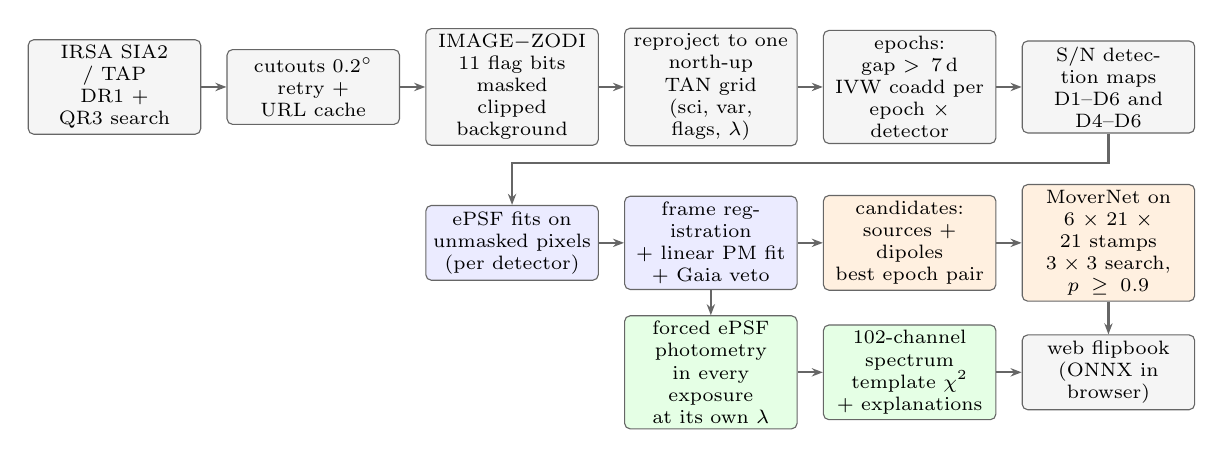
\begin{tikzpicture}[
  font=\scriptsize,
  box/.style={draw=black!60, rounded corners=2pt, fill=#1, align=center, minimum height=0.95cm,
              text width=2.05cm, inner sep=2pt},
  box/.default=white,
  arr/.style={-{Stealth[length=4pt]}, thick, black!60},
  node distance=0.32cm and 0.32cm]
  % ingest row
  \node[box=black!4] (sia) {IRSA SIA2 / TAP\\DR1 + QR3 search};
  \node[box=black!4, right=of sia] (cut) {cutouts 0.2$^\circ$\\retry + URL cache};
  \node[box=black!4, right=of cut] (cal) {IMAGE$-$ZODI\\11 flag bits masked\\clipped background};
  \node[box=black!4, right=of cal] (rep) {reproject to one\\north-up TAN grid\\(sci, var, flags, $\lambda$)};
  \node[box=black!4, right=of rep] (ep) {epochs: gap $>7$\,d\\IVW coadd per\\epoch $\times$ detector};
  \node[box=black!4, right=of ep] (snr) {\SN{} detection maps\\D1--D6 and D4--D6};
  % branches (columns line up with the row above)
  \node[box=blue!8, below=0.75cm of cal] (ast) {ePSF fits on\\unmasked pixels\\(per detector)};
  \node[box=blue!8, right=of ast] (reg) {frame registration\\+ linear PM fit\\+ Gaia veto};
  \node[box=orange!12, right=of reg] (cand) {candidates:\\sources + dipoles\\best epoch pair};
  \node[box=orange!12, right=of cand] (cnn) {MoverNet on\\$6\times21\times21$ stamps\\$3\times3$ search, $p\geq0.9$};
  \node[box=green!10, below=0.32cm of reg] (fp) {forced ePSF photometry\\in every exposure\\at its own $\lambda$};
  \node[box=green!10, right=of fp] (bin) {102-channel spectrum\\template $\chi^2$\\+ explanations};
  \node[box=black!4, right=of bin] (web) {web flipbook\\(ONNX in browser)};
  \draw[arr] (sia) -- (cut);
  \draw[arr] (cut) -- (cal);
  \draw[arr] (cal) -- (rep);
  \draw[arr] (rep) -- (ep);
  \draw[arr] (ep) -- (snr);
  \draw[arr] (snr.south) -- ++(0,-0.37) -| (ast.north);
  \draw[arr] (ast) -- (reg);
  \draw[arr] (reg) -- (cand);
  \draw[arr] (cand) -- (cnn);
  \draw[arr] (reg) -- (fp);
  \draw[arr] (fp) -- (bin);
  \draw[arr] (bin) -- (web);
  \draw[arr] (cnn) -- (web);
\end{tikzpicture}
\caption{The Blink pipeline. Grey: data preparation (\S\ref{sec:epochs}). Blue: astrometry
(\S\ref{sec:astrometry}). Orange: machine-learning motion detection (\S\ref{sec:cnn},\ref{sec:candidates}).
Green: spectroscopy and classification (\S\ref{sec:spectra}). Every arrow operates on real data only;
synthetic injections exist solely inside the training set.}
\label{fig:pipeline}
\end{figure*}

\paragraph{Calibration and resampling.} For every exposure we subtract the provided zodiacal model and
mask pixels carrying any of eleven \texttt{FLAGS} bits (transient, overflow, non-functional, dichroic,
missing data, hot, cold, non-linear, persistence, outlier, sur-error). A $3\sigma$-clipped median removes
residual background. All exposures are then resampled onto a single north-up gnomonic grid centred on the
target at the native 6.15\asec{} scale; the output-to-input pixel map is computed once and reused for the
science and variance planes (bilinear), the flags (nearest neighbour, so bits are never blended) and the
wavelength plane (bilinear). Bilinear resampling deliberately propagates NaNs to neighbours, a conservative
mask growth. For named targets, the grid is centred on the proper-motion-propagated 2026.0 position:
\wise's catalogue position is from $\sim$2010 and it has moved $\sim$2\amin{} since.

\paragraph{Epochs for an LVF survey.} A SPHEREx visit steps a field through the LVF over $\sim$3 weeks, and
visits recur every $\sim$6 months. We define an epoch as a maximal run of exposures with no gap longer than
7 days. Within an epoch $e$ and detector $d$ we form the inverse-variance weighted coadd
\begin{equation}
  \hat I_{ed} = \frac{\sum_{i\in(e,d)} I_i/\sigma_i^2}{\sum_{i\in(e,d)} 1/\sigma_i^2},
  \qquad
  \hat\sigma^2_{ed} = \Big(\sum_{i\in(e,d)} 1/\sigma_i^2\Big)^{-1},
\end{equation}
which averages over the wavelengths that detector sampled in that visit. Epochs with fewer than six
exposures (or fewer than three in a detector) are ``short visits''; they are single-wavelength snapshots
and are excluded from astrometry and hidden by default in the viewer.

\paragraph{Combining detectors in \SN{} space.} The six detectors observe at different wavelengths and in
different surface-brightness units, so we never add their fluxes. Instead, the detection image for a set of
detectors $\mathcal D$ is
\begin{equation}
  S_{\mathcal D}(\mathbf x) = \frac{1}{\sqrt{k(\mathbf x)}}\sum_{d\in\mathcal D}
      \frac{\hat I_{d}(\mathbf x)}{\hat\sigma_{d}(\mathbf x)},
  \label{eq:snr}
\end{equation}
where $k$ counts the detectors with valid data at $\mathbf x$, so $S$ is in units of $\sigma$ for pure noise
regardless of spectrum. We build two such images: $\mathcal D=\{1..6\}$ for general detection and the
\emph{red} set $\mathcal D=\{4,5,6\}$ (2.4--5\,\um), where Y dwarfs emit nearly all of their flux and
bluer field stars are fainter. The same construction is used for difference images,
replacing $\hat I_d$ by $\hat I^{B}_d-\hat I^{A}_d$ and $\hat\sigma^2_d$ by
$\hat\sigma^{2,A}_d+\hat\sigma^{2,B}_d$, which compares each detector with itself before combining and
so cancels the chromatic term that a naive multi-band difference would leave.

% ================================================================ 4. astrometry
\section{Masked-pixel ePSF astrometry}
\label{sec:astrometry}

\paragraph{Model.} Sources are local maxima of $S$ above $7\sigma$ (D1--D6) or $6\sigma$ (D4--D6).
Saturated stars appear as compact masked islands ringed by \SN{}$>15$; we detect these separately and
suppress the ring of spurious peaks around them. For each source, epoch and detector we fit
\begin{equation}
  m(x,y) = F\,P_{ed}(x-x_0,\,y-y_0) + b
\end{equation}
by weighted least squares over a $9\times9$ box ($13\times13$ for saturated stars), \emph{using only
unmasked pixels}. $P_{ed}$ is the mean of the \texttt{EPSF} zones of the exposures in the coadd, sampled
from the $\times5$ oversampled grid with bilinear interpolation; its spatial gradient is precomputed, so
the Jacobian columns $\big[P,\,1,\,-F\partial_xP,\,-F\partial_yP\big]$ are analytic. We take
Levenberg--Marquardt-damped Gauss--Newton steps ($\lambda=10^{-3}$, steps clipped to 0.5\,px, at most
12 iterations, $\sim$1\,ms per fit). Because the masked core simply drops out of the likelihood, the fit
constrains a saturated star's position from the PSF wings---the only way to measure Barnard's Star, whose
core is masked in every exposure. Covariances are scaled by $\max(\chisqnu,1)$.

\paragraph{Combining detectors.} Per-detector positions with $\sigma>0.6$\,px or flux \SN{}$<5$ are
rejected. The rest are combined by inverse variance, and the uncertainty is inflated to the empirical
scatter between detectors,
\begin{equation}
  \sigma_x = \max\!\Big(\big(\textstyle\sum_d \sigma_{x,d}^{-2}\big)^{-1/2},\;
                         \mathrm{std}_d(x_d)/\sqrt{n_d}\Big),
\end{equation}
which absorbs chromatic PSF differences and the fact that the ePSF (defined in detector coordinates) is
applied un-rotated on our north-up grid.

\paragraph{Registration and motion.} Small per-epoch frame offsets are removed by iteratively solving for
the translation that keeps the ensemble of well-measured sources ($\sigma<0.25$\,px) fixed, using the
$3\times$NMAD-clipped median displacement. Each source then gets a weighted linear fit
$x(t)=a+\mu_x(t-t_\mathrm{ref})$ with per-epoch variance $\sigma^2+\sigma_\mathrm{sys}^2$ and a systematic
floor $\sigma_\mathrm{sys}=0.025$\,px; errors are scaled by $\sqrt{\max(\chisqnu,1)}$. A source is a
\emph{significant mover} if $\mu/\sigma_\mu\geq5$ with at least three epochs.

\paragraph{Red de-blending.} The red (D4--D6) pass is matched to the full pass within 1.5\,px; when the
red measurement is a more significant mover it replaces the full-band one, which is otherwise biased by a
bluer blended neighbour.

\paragraph{Gaia veto.} A significant mover matched (within 4\asec) to a Gaia source that Gaia measures to be
nearly static ($\mu_\mathrm{G}<0.3\mu$ and $|\mu-\mu_\mathrm{G}|>2.5\sigma_\mu$) is reported as
``rejected by Gaia'' rather than as a mover. In the five fields this fired twice, both in the \epsIndiB{}
field.

\paragraph{Wing photometry.} For saturated cores we also provide relative light curves from the
background-subtracted flux in an annulus just outside the masked core. Within one detector the wings scale
with the total flux, so the light curve is valid in a relative sense, though not calibrated to \uJy.

% ================================================================ 5. CNN
\section{MoverNet: learning motion from injections into real data}
\label{sec:cnn}

Centroid motion fails exactly where discovery matters most: for faint objects, and for movers that
are blended with a static star. We therefore train a classifier that looks at pixels directly, in the
spirit of the real/bogus networks used by transient surveys \citep{duev2019}.

\paragraph{Input representation.} A sample is a $6\times21\times21$ stamp ($\sim$2\amin{} on a side)
centred on a candidate position for a pair of epochs $(A,B)$:
\begin{equation}
  \mathbf X = \big[S^A_{1..6},\,S^B_{1..6},\,S^{B-A}_{1..6},\;
                   S^A_{4..6},\,S^B_{4..6},\,S^{B-A}_{4..6}\big],
\end{equation}
each built with Eq.~\eqref{eq:snr}. The two colour groups let the network see a Y dwarf that is invisible
in the full-band channels but obvious in the red ones. A robust plane $a+bx+cy$ (iteratively fitted with
$2.5\times$MAD clipping so sources do not bias it) is subtracted from each channel, removing large-scale
background gradients between epochs, and the dynamic range of bright stars (\SN{}$\sim10^3$) is
compressed with $\tilde{\mathbf X}=\operatorname{asinh}(\mathbf X/3)$.

\paragraph{Positives: physically calibrated injections.} We draw a speed $v\sim\log\mathcal U(0.3,15)$\asecyr,
a direction, a total \SN{} $s\sim\log\mathcal U(3,400)$, and a spectral shape: flat, \emph{red} (Y/T-dwarf
like, with relative per-detector amplitudes $w=(0,0.02,0.08,0.5,1,1)$ for D1--D6) or \emph{blue}
(stellar Rayleigh--Jeans tail). The per-detector target \SN{} is $s_d=s\,w_d/\lVert w\rVert$, so the
combined \SN{} of Eq.~\eqref{eq:snr} is $\approx s$. A point source is then added to \emph{each real
epoch-detector coadd} using \emph{that coadd's own ePSF} $P_{ed}$ at linearly-moving positions
$\mathbf x_A$ and $\mathbf x_B=\mathbf x_A+v\,\Delta t\,\hat{\mathbf n}$, with flux chosen so that its
optimal (PSF-weighted) \SN{} is exactly $s_d$:
\begin{equation}
  F_{ed} = \frac{s_d}{\sqrt{\sum_{\mathbf p} P_{ed}(\mathbf p-\mathbf x)^2/\hat\sigma^2_{ed}(\mathbf p)}}.
  \label{eq:inject}
\end{equation}
Equation~\eqref{eq:inject} makes injected \SN{} meaningful in every detector, every epoch and every
noise environment, including masked pixels and depth variations. A small lognormal brightness change
($\sigma_{\ln}=0.15$) between epochs prevents the network from relying on exact flux conservation. Only
epoch pairs at least 0.35\,yr apart are used, and injections that move less than 0.35\,px are discarded:
such ``positives'' are physically indistinguishable from static sources and act as label noise
(\S\ref{sec:ablation}). The stamp centre is jittered by $\mathcal N(0,0.7^2)$\,px around the track midpoint.

\paragraph{Adversarial negatives.} The negative class is designed so that \emph{anything that changes but
does not move} is a negative:
\begin{itemize}
  \item \emph{static sources} (28\%): real detected sources, jittered;
  \item \emph{static variables} (18\%): synthetic sources injected at the \emph{same} position in both
        epochs with a flux ratio $\log\mathcal U(1.5,8)^{\pm1}$---the RW~Aur/R~Dra case;
  \item \emph{difference peaks} (18\%): real $|S^{B-A}|>4.5\sigma$ pixels, i.e.\ artefacts, real variables
        and saturated-star residuals;
  \item \emph{off-centre movers} (20\%): real-looking injected movers placed 4--9\,px from the stamp centre,
        so the label refers to the \emph{centre} and the network cannot answer ``is there a dipole
        anywhere?'';
  \item \emph{saturated-star edges} (6\%) and \emph{empty sky} (10\%).
\end{itemize}
Known movers and every Gaia star faster than 0.3\asecyr{} are masked (within 8--10\,px) from all training
sites, so real movers are \emph{test-only}.

\paragraph{Architecture and training.} MoverNet is a five-layer CNN (Conv-BN-ReLU blocks of width
24, 24, 48, 48, 64 with two max-pools, global average pooling, dropout 0.3, and a 64--32--1 head;
67{,}969 parameters). It is trained with binary cross-entropy, AdamW (weight decay $10^{-4}$) and a
one-cycle schedule (peak learning rate $3\times10^{-3}$) for 16 epochs at batch size 256, with the eight
dihedral (rotation/flip) augmentations, on CPU in minutes. The training set has 36{,}000 balanced stamps from
13 fields; the test set has 4{,}800 stamps from the two held-out fields. The model is exported to ONNX
(opset 17; outputs checked against PyTorch on random inputs at export) and runs unchanged in the
browser via onnxruntime-web.

% ================================================================ 6. candidates
\section{Calibrated field search}
\label{sec:candidates}

\paragraph{Epoch pair.} For a field we pick the pair maximising
$\Delta t \times \overline{\mathrm{median}(1/\hat\sigma)}$, trading motion signal (baseline) against depth.

\paragraph{Candidates.} Two complementary generators feed the classifier: (1) every detected source,
centred on its motion-model midpoint between the two epochs (static if $\mu/\sigma_\mu<3$); and
(2) every \emph{difference dipole}---a positive and a negative $|S^{B-A}|>4\sigma$ peak 0.7--4.5\,px
apart---centred on the dipole midpoint, \emph{even if it overlaps a catalogued source}. The second channel
exists for the case centroiding cannot handle: a mover passing a static star, as \wise{} does in 2025--26.

\paragraph{Local search and threshold calibration.} A blended or static-fit centroid can miss a track
midpoint by $\sim$1\,px, so each candidate is scored on a $3\times3$ grid of $\pm1$\,px offsets and the
maximum is kept. Taking the best of nine scores inflates the false-positive rate relative to the
single-stamp model card, so we recalibrate the decision threshold on real data: at $p\geq0.9$, only
0.6\% of 628 static Gaia stars in the challenge fields are flagged.

% ================================================================ 7. spectra
\section{Spectra of moving positions and ``what is it?''}
\label{sec:spectra}

\paragraph{Forced exposure-level photometry.} Because every exposure samples a different wavelength at
the source, the spectrum is assembled from the exposures themselves rather than from coadds. For a
(possibly moving) sky position we propagate the motion model to each exposure's mid-time, read the
wavelength $\lambda_i$ from the resampled \texttt{WCS-WAVE} plane at that pixel, and fit the flux with the
exposure's own ePSF at the \emph{fixed} model position (no centroid freedom, so faint exposures are not
biased upward). Fluxes are converted to \uJy{} with the pixel solid angle,
$\Omega_\mathrm{pix}=(6.15\asec)^2$. Measurements are binned into the 102 SPHEREx channels of
\citet{gagne2026} by inverse-variance weighting; when a channel has $\geq3$ measurements its error is
inflated to the scatter between them, absorbing variability and residual systematics.

\paragraph{Template families.} We fit (i) the 47 SPIFF SPHEREx brown-dwarf standards, M8--Y1 including
young ($\beta$, $\gamma$, $\delta$) and subdwarf variants \citep{gagne2026}; (ii) Planck spectra for stars,
2600--30{,}000\,K; and (iii) power laws $f_\nu\propto\lambda^\beta$ as a deliberately simple galaxy/QSO
family. Each template has a free analytic scale, and the variance is
$\sigma^2+(0.03f)^2+(a\,\sigma_\mathrm{tmpl})^2$, i.e.\ a 3\% calibration floor plus the template's own
uncertainty. Solar-system membership is decided by motion (a SkyBoT match at the time of the visit),
not by colour.

\paragraph{Tempered probabilities.} Writing $\chi^2_f$ for the best template in family $f$, we report
\begin{equation}
  p_f \propto \exp\!\left[-\frac{\chi^2_f-\chi^2_\mathrm{min}}{2T}\right],\qquad
  T=\max\!\big(\chi^2_\mathrm{min}/\nu,\,1\big),
\end{equation}
so that a poor-but-best fit (a blend, a variable, an object outside the library) does not produce a
spuriously confident answer.

\paragraph{Explanations.} To show \emph{why} an object is classified as it is, we split the spectrum into
ten physically labelled regions (water at 1.4, 1.9 and 2.7\,\um, methane at 1.6 and 3.3\,\um, the
4.5\,\um{} peak and CO at 4.6\,\um, \ldots) and report the per-region
$\Delta\chi^2=\chi^2_\mathrm{runner\text{-}up}-\chi^2_\mathrm{best}$ between the two leading families,
together with classic water and methane indices.

% ================================================================ 8. results
\section{Results}
\label{sec:results}

\subsection{Astrometry against Gaia DR3}

Figure~\ref{fig:gaia} compares our proper-motion components with Gaia DR3 for the 468 sources with
$\geq3$ epochs and a Gaia match. The median residual is 7\,\masyr{} and the robust scatter is
127\,\masyr{} per component, i.e.\ $\approx0.02$\,px\,yr$^{-1}$ at SPHEREx resolution after only
$\sim$1.4\,yr of data. The normalised residuals have a median of 0.03 and an NMAD of 0.42: our
uncertainties are \emph{conservative} by a factor of $\sim$2.4, mostly because of the $\chisqnu$ scaling and
systematic floor, and 99.9\% of components lie within $3\sigma$ of Gaia. For the two fast targets
(Table~\ref{tab:movers}) we recover Barnard's Star at $10.11\pm1.53$\asecyr{} (Gaia 10.39; $0.2\sigma$),
measured entirely from the wings of a core that is saturated in every exposure, and \epsIndiB{} at
$5.04\pm0.39$\asecyr{} (Gaia 4.68; $0.9\sigma$; $12.8\sigma$ detection). Both were measured in the red
(D4--D6) pass.

\wise{} is \emph{not} recovered by centroiding: in 2025--26 it passes within $\sim$1\,px of a background
star, and the PSF fit locks onto the blend. It is nevertheless visible in D5/D6 at 8--12$\sigma$ per epoch
and as a dipole in the difference image (Fig.~\ref{fig:motion})---the case MoverNet was built for.

\begin{figure*}[t]
\centering
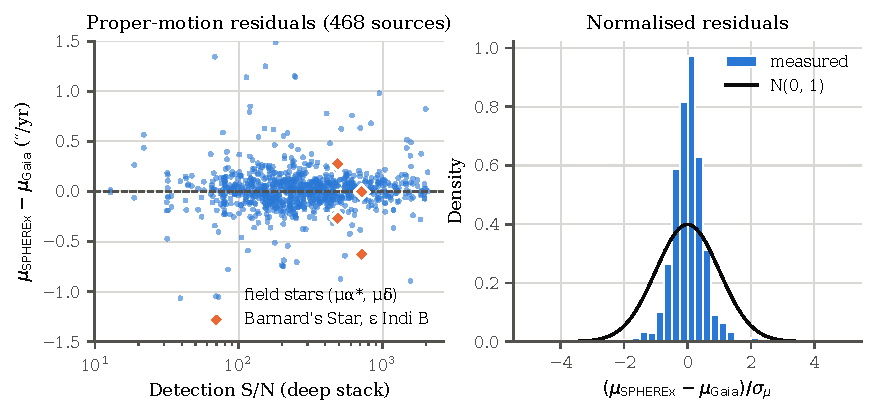
\includegraphics[width=\textwidth]{gaia_pm.pdf}
\caption{Proper motions against Gaia DR3 in the five challenge fields. \emph{Left:} per-component residuals
versus detection \SN{}; diamonds are Barnard's Star and \epsIndiB. \emph{Right:} residuals normalised by our
uncertainties, compared with a unit Gaussian; the narrower distribution shows that our errors are
conservative.}
\label{fig:gaia}
\end{figure*}

\begin{table}[t]
\centering
\caption{Known movers in the challenge fields. $\mu$: our total proper motion; $p$: MoverNet score of the
best-of-nine stamp; rank: position of the object in its field's candidate list.}
\label{tab:movers}
\small
\setlength{\tabcolsep}{3pt}
\begin{tabular}{@{}lccccc@{}}
\toprule
Object & $\mu$ (\asecyr) & Gaia & $p$ & Rank & $N_\mathrm{cand}$ \\
\midrule
Barnard's Star & $10.11\pm1.53$ & 10.39 & 1.00 & 1 & 293 \\
\epsIndiB      & $5.04\pm0.39$  & 4.68  & 1.00 & 1 & 156 \\
\wise          & blended        & ---$^a$ & 0.97 & 2 & 168 \\
\bottomrule
\end{tabular}\\[2pt]
\footnotesize $^a$ Not in Gaia; catalogue $\mu=8.15$\asecyr.
\end{table}

\subsection{MoverNet on held-out fields}

On the 4{,}800 stamps from GOODS-N and Plane-1, which the network never saw, MoverNet reaches
ROC AUC 0.873 and average precision 0.895 (Fig.~\ref{fig:roc}); at $p\geq0.5$ the precision is 0.865 and
the recall 0.674 (1617 TP, 253 FP, 783 FN). Recall is similar for flat (0.69) and red (0.69) spectra and
lower for blue (0.62) spectra. False-positive rates by negative type are 7.9\% (off-centre
movers), 9.9\% (static sources), 10.5\% (difference peaks), 12.5\% (empty sky) and 13.2\% (static
variables).

The completeness map (Fig.~\ref{fig:completeness}) behaves as expected: recovery rises with \SN{}, from
23--42\% at \SN{}$<5$ to 93--98\% at \SN{}$>100$, and with displacement, with sub-pixel motions
(0.35--0.6\,px) the hardest. At \SN{}$=20$--40, a mover displaced by 1.5--2.5\,px---Barnard's-Star-like
speeds over a year---is recovered 78\% of the time.

\begin{figure*}[t]
\centering
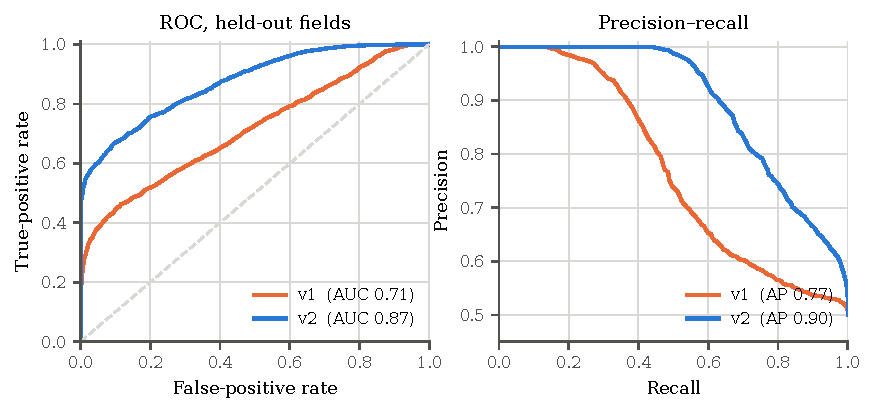
\includegraphics[width=\textwidth]{roc_pr.pdf}
\caption{ROC and precision--recall curves on the two held-out fields for the first (v1) and final (v2)
MoverNet. Changes between the two are listed in Table~\ref{tab:ablation}.}
\label{fig:roc}
\end{figure*}

\begin{figure}[t]
\centering
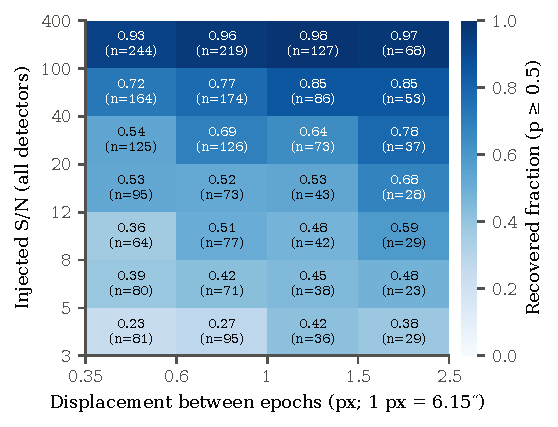
\includegraphics[width=\columnwidth]{completeness.pdf}
\caption{Fraction of injected movers in the held-out fields recovered at $p\geq0.5$, as a function of
injected \SN{} and displacement between the two epochs. Cell labels give the fraction and the number
of injections.}
\label{fig:completeness}
\end{figure}

\subsection{Real objects never trained on}

The decisive test uses real objects. We score the three known movers and 606 bright static Gaia stars
($\mu_\mathrm{G}<20$\,\masyr, \SN{}$>8$) on single stamps at their Gaia-propagated track midpoints
(Fig.~\ref{fig:realscores}). Barnard's Star scores 0.99, \epsIndiB{} 1.00 and \wise{} 0.97, while only
1.7\% of static stars reach 0.5. The two variable stars score 0.13 (R~Dra) and 0.49 (RW~Aur): both below
the field threshold, but RW~Aur shows that strong variability remains the most mover-like contaminant.
Figure~\ref{fig:stamps} shows the actual network inputs: Barnard's Star appears as a large dipole around
a masked core, \epsIndiB{} as a clean dipole in both colour groups, and \wise{} as a faint dipole beside a
brighter static neighbour. The bottom row is the highest-scoring static star in the RW~Aur field---a bright
star whose PSF-mismatch residual forms a ring rather than a dipole---illustrating the hardest negatives.

In full field searches (\S\ref{sec:candidates}), the three movers rank \#1, \#1 and \#2 among 293, 156
and 168 candidates respectively (Table~\ref{tab:movers}). The two variable-star fields produce 2 (RW~Aur) and 0 (R~Dra)
candidates above the threshold; the remaining above-threshold candidates in the three mover fields
(3, 1 and 4) have not yet been vetted.

\begin{figure*}[t]
\centering
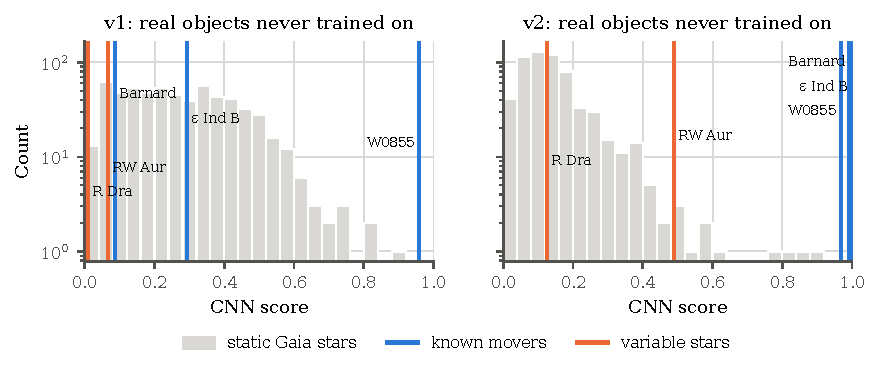
\includegraphics[width=\textwidth]{real_scores.pdf}
\caption{MoverNet scores of real objects that were masked from training: 606 static Gaia stars (histogram,
log scale), three known movers (blue) and two variable stars (orange), for the first (left) and final
(right) networks.}
\label{fig:realscores}
\end{figure*}

\begin{figure}[t]
\centering
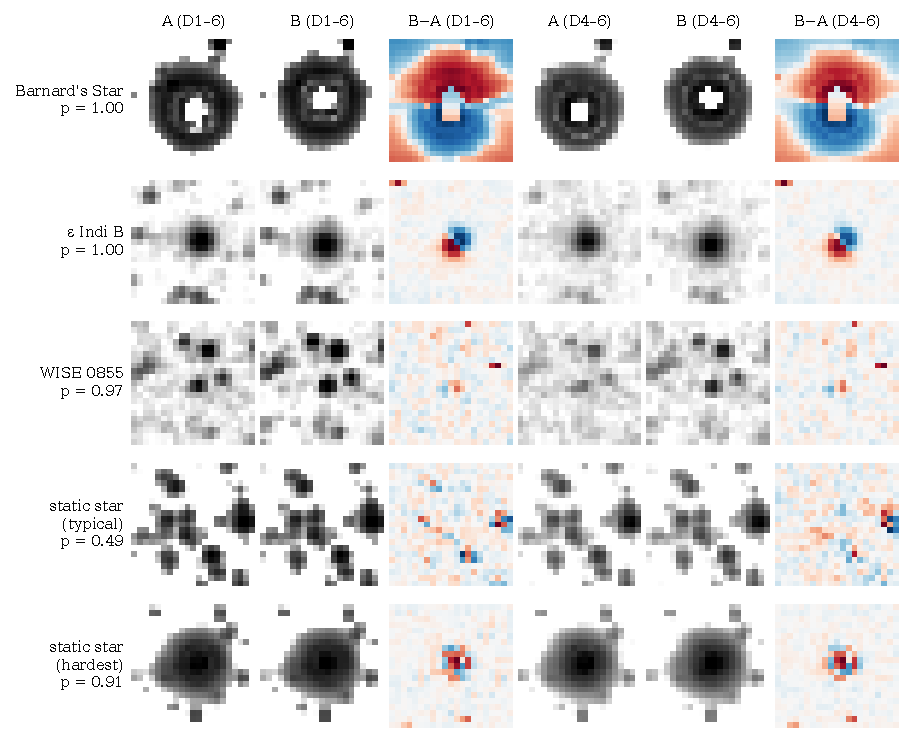
\includegraphics[width=\columnwidth]{stamps.pdf}
\caption{MoverNet inputs for real candidates ($\operatorname{asinh}$-stretched \SN{}; difference channels
in red/blue). Rows: the three known movers and two static stars from the RW~Aur field, a typical one and
the highest-scoring one.}
\label{fig:stamps}
\end{figure}

\begin{figure*}[t]
\centering
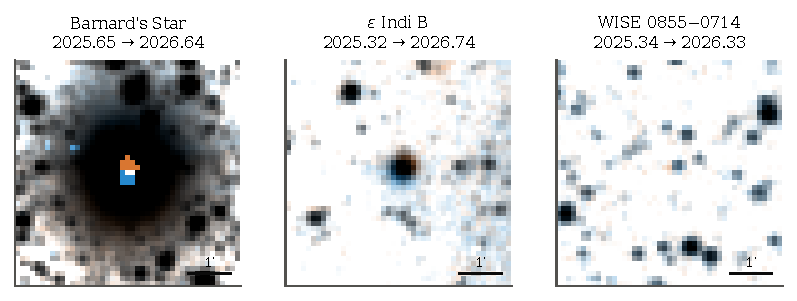
\includegraphics[width=\textwidth]{motion.pdf}
\caption{``Motion'' view of the red (D4--D6) detection images for the best epoch pair, as rendered by the
Blink viewer (inverted for print): epoch $A$ in blue and epoch $B$ in orange, so static sources are neutral
and movers split in colour. Barnard's Star is saturated, and its masked core is drawn per epoch.
\wise{} (centre of the right panel) moves past a background star and is not resolved by centroiding.}
\label{fig:motion}
\end{figure*}

\subsection{Spectral classification}

Figure~\ref{fig:spectrum} shows the spectrum of \epsIndiB{} assembled from 454 exposures into 101 channels.
The deep water bands at 1.4 and 1.9\,\um, methane at 3.3\,\um{} and the strong 4\,\um{} peak are obvious.
The best template is a T2 standard ($\chisqnu=4.5$; T4 and T3 follow at 5.4), against 314 for the best
blackbody and 159 for the best power law, giving $p_\mathrm{BD}=1.00$. The regions that drive the
decision are 3.7--4.2\,\um{} ($\Delta\chi^2=2793$), 1.5--1.8\,\um{} (2457), 0.75--1.1\,\um{} (1455) and
4.2--5.0\,\um{} (1453). \epsIndiB{} is an unresolved T1+T6 binary \citep{mccaughrean2004}, so a composite
early/mid-T spectrum is the expected answer. For \wise{} the classifier returns ``brown dwarf, $\sim$T5'':
correctly a brown dwarf but too early, because the true type (Y4; \citealt{kirkpatrick2021}) lies beyond the
library's coolest Y1 standard and its short-wavelength photometry is blended. Bright field stars are
classified as $\sim$5000\,K stars. Saturated stars get no spectrum.

\begin{figure*}[t]
\centering
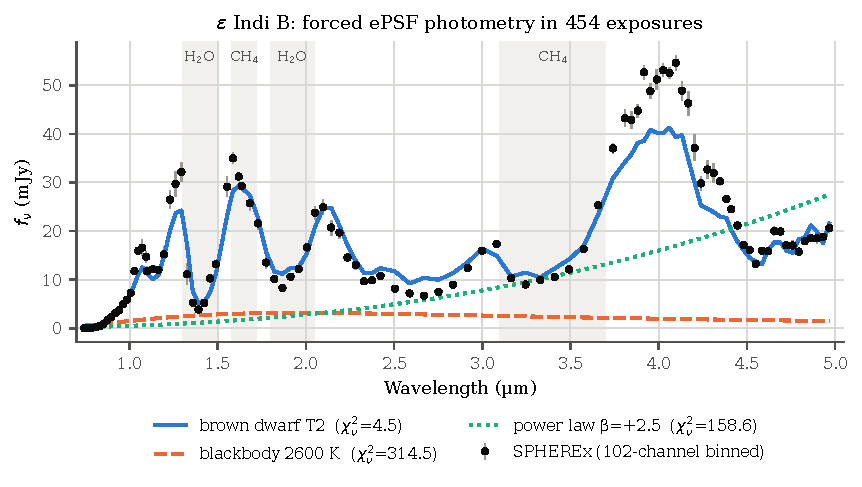
\includegraphics[width=\textwidth]{spectrum_epsindib.pdf}
\caption{SPHEREx spectrum of \epsIndiB{} from forced ePSF photometry in every exposure at its own LVF
wavelength, binned to the 102 SPHEREx channels, with the best template in each family. Shaded:
molecular bands.}
\label{fig:spectrum}
\end{figure*}

% ================================================================ 9. ablation
\section{Ablation: what made the network work}
\label{sec:ablation}

Our first network (v1) used the same architecture and input representation but a naive training set.
On held-out fields it reached only AUC 0.71, and on real data it \emph{missed} Barnard's Star (0.09) and
\epsIndiB{} (0.29). Its training curves (Fig.~\ref{fig:training}) look healthy, which is the point: in-distribution
validation accuracy did not reveal the problem; only held-out fields and real objects did.
Diagnosing these failures led to five changes (Table~\ref{tab:ablation}):
\begin{enumerate}
  \item \textbf{Epoch pairs $\geq0.35$\,yr apart and displacements $\geq0.35$\,px.} v1 drew pairs that could
        be weeks apart within one survey visit, creating ``movers'' that had not moved: unlearnable
        positives that taught the network to be uncertain everywhere.
  \item \textbf{Off-centre movers as negatives.} v1 learned ``there is a dipole somewhere in the stamp''
        and fired on neighbours of movers.
  \item \textbf{\SN{} range extended from 60 to 400.} v1 had never seen a bright mover and so scored the two
        brightest real movers as static.
  \item \textbf{Robust plane (not median) background per channel}, removing epoch-to-epoch gradients that v1
        flagged as change.
  \item \textbf{A threshold calibrated on real static stars} for the best-of-nine local search.
\end{enumerate}
Because the v1 and v2 test sets were generated with their own recipes, their held-out metrics are
indicative; the real-object test, however, uses the identical 606 stars and five targets for both
networks and is a like-for-like comparison. There, the false-positive rate on static stars fell
fivefold (8.7\%$\to$1.7\%) while both bright movers went from missed to $p\geq0.99$. The cost is visible
too: RW~Aur rose from 0.07 to 0.49, so v2 trades some robustness to strong variables for sensitivity to
bright movers.

\begin{table}[t]
\centering
\caption{v1 vs.\ v2 MoverNet (same architecture). Held-out metrics at $p\geq0.5$; ``static FP'' is the
fraction of 606 real static Gaia stars with $p\geq0.5$.}
\label{tab:ablation}
\small
\begin{tabular}{@{}lcc@{}}
\toprule
 & v1 & v2 \\
\midrule
Training stamps & 28{,}000 & 36{,}000 \\
ROC AUC (held-out) & 0.713 & \textbf{0.873} \\
Average precision & 0.767 & \textbf{0.895} \\
Precision / recall & 0.82 / 0.43 & \textbf{0.86 / 0.67} \\
Static FP (real) & 8.7\% & \textbf{1.7\%} \\
\midrule
Barnard's Star & 0.09 & \textbf{0.99} \\
\epsIndiB      & 0.29 & \textbf{1.00} \\
\wise          & 0.96 & \textbf{0.97} \\
R Dra (variable) & \textbf{0.01} & 0.13 \\
RW Aur (variable) & \textbf{0.07} & 0.49 \\
\bottomrule
\end{tabular}
\end{table}

\begin{figure}[t]
\centering
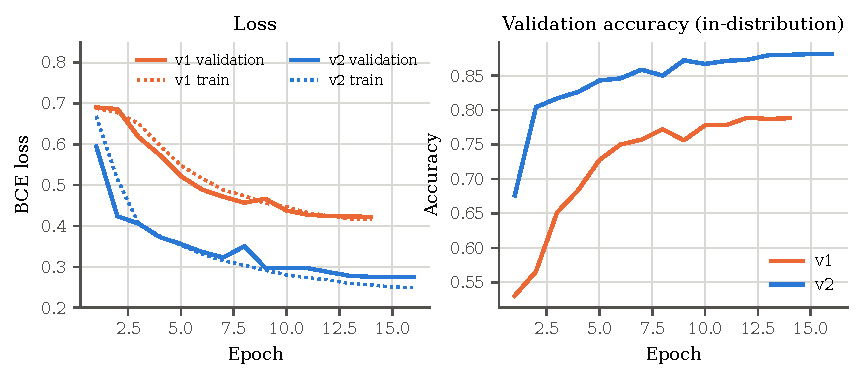
\includegraphics[width=\columnwidth]{training.pdf}
\caption{Training curves for v1 and v2 (validation split drawn from the training fields).}
\label{fig:training}
\end{figure}

% ================================================================ 10. system
\section{The Blink application}
\label{sec:app}

Blink is a FastAPI back end and a Next.js front end. Any sky position is a URL; the five challenge targets
ship as static snapshots so the viewer works offline, and any other position is built on demand
(1--5 minutes on first request, then cached). Flipbook frames are sent as float32 arrays and stretched in
the browser (asinh, log or linear) with \emph{one set of levels shared by all frames}, so that blinking is
honest: a source cannot appear to vary because of per-frame normalisation. Views include the flipbook,
the inverse-variance stack, the difference image (per-detector \SN{}, $|\Delta|<1.5\sigma$ suppressed) and
the two-colour motion view (Fig.~\ref{fig:motion}). Masked pixels are drawn in a distinct colour rather than
black, so saturated cores do not read as dark holes. Light curves are shown per detector, with short visits
drawn hollow, because the LVF alone can mimic variability across detectors. The top 60 candidates ship with
their stamps and are re-scored client-side with onnxruntime-web, so users can verify the network's output
without the server. IRSA services returned intermittent 5xx errors throughout development; every request
retries with backoff and is cached on disk keyed by URL.

% ================================================================ 11. limitations
\section{Limitations and future work}
\label{sec:limits}

\begin{itemize}
  \item \textbf{Linear motion only.} We fit no parallax. For the nearest objects (Barnard's Star 0.55\asec,
        \wise{} 0.44\asec) the annual parallax is a sizeable fraction of a pixel and, with a six-month
        cadence, aliases into the motion fit. A five-parameter astrometric solution is the natural next
        step as more surveys accumulate.
  \item \textbf{Un-rotated ePSF.} The ePSF is defined in detector coordinates; we apply it on a north-up
        grid. SPHEREx PSFs are nearly round, so this mainly costs precision, which our error inflation absorbs.
  \item \textbf{Two-epoch classifier.} MoverNet sees one epoch pair. A sequence model over all epochs
        would gain $\sqrt{N}$ in depth and could reject variables by their light curve.
  \item \textbf{Template coverage.} Stars are blackbodies, which cannot capture M-dwarf water bands, and the
        brown-dwarf library ends at Y1, which biases the coldest objects to earlier types.
  \item \textbf{Completeness.} Recall below \SN{}$\approx12$ is 23--59\%; a dedicated low-\SN{} detection
        channel (e.g.\ shift-and-stack along trial velocities) would extend the reach of the search toward
        the faint, slow objects a Planet~X search requires.
  \item \textbf{Data volume.} The present system processes $12\amin$ fields; the methods are local and
        embarrassingly parallel, so an all-sky run is an engineering, not a methodological, problem.
\end{itemize}

% ================================================================ 12. conclusion
\section{Conclusion}

SPHEREx was built to measure spectra, not motions, but its six-month all-sky cadence makes it a
blink comparator for the infrared sky. We showed that with an LVF-aware epoch model, masked-pixel ePSF
astrometry and a classifier trained purely on physically calibrated injections into real data, the
public DR1+QR3 images already recover every known high-proper-motion object in the challenge fields at the
top of their candidate lists---including one that classical centroiding misses---and assign each a
102-channel spectrum and an explained classification. Every number in this paper is regenerated from the
pipeline's data products by a single script.

% ================================================================ back matter
\section*{Acknowledgments}
This work uses data from SPHEREx, a NASA Medium-Class Explorer, served by the NASA/IPAC Infrared Science
Archive; data from the European Space Agency mission Gaia, processed by the Gaia Data Processing and
Analysis Consortium; the SkyBoT and Sesame services of the CDS; and the SPIFF SPHEREx brown-dwarf templates
of \citet{gagne2026} (CC BY 4.0). Software: Astropy \citep{astropy2022}, NumPy, SciPy, PyTorch
\citep{paszke2019}, ONNX Runtime, FastAPI and Next.js. Software development was assisted by an AI coding
assistant; all results were produced by, and can be regenerated from, the released code.

\section*{Code and data availability}
The pipeline, trained model (\texttt{ml/models/mover.onnx}), metrics and the script that produces every
figure in this paper (\texttt{paper/make\_figures.py}) are included in the Blink repository.

\begin{thebibliography}{99}
\setlength{\itemsep}{1pt}
\small

\bibitem[{Astropy Collaboration}(2022)]{astropy2022}
Astropy Collaboration, Price-Whelan, A.~M., et al. 2022, ApJ, 935, 167

\bibitem[{Batygin \& Brown}(2016)]{batygin2016}
Batygin, K., \& Brown, M.~E. 2016, AJ, 151, 22

\bibitem[{Berthier et al.}(2006)]{berthier2006}
Berthier, J., Vachier, F., Thuillot, W., et al. 2006, in ASP Conf.\ Ser.\ 351, Astronomical Data Analysis
Software and Systems XV, 367

\bibitem[{Crill et al.}(2020)]{crill2020}
Crill, B.~P., Werner, M., Akeson, R., et al. 2020, Proc.\ SPIE, 11443, 114430I

\bibitem[{Dor\'e et al.}(2014)]{dore2014}
Dor\'e, O., Bock, J., Ashby, M., et al. 2014, arXiv:1412.4872

\bibitem[{Duev et al.}(2019)]{duev2019}
Duev, D.~A., Mahabal, A., Masci, F.~J., et al. 2019, MNRAS, 489, 3582

\bibitem[{Gagn\'e et al.}(2026)]{gagne2026}
Gagn\'e, J., et al. 2026, SPIFF: SPHEREx spectral standards of ultracool dwarfs, Zenodo,
doi:\href{https://doi.org/10.5281/zenodo.19051216}{10.5281/zenodo.19051216}

\bibitem[{Gaia Collaboration}(2023)]{gaia2023}
Gaia Collaboration, Vallenari, A., Brown, A.~G.~A., et al. 2023, A\&A, 674, A1

\bibitem[{Kirkpatrick et al.}(2021)]{kirkpatrick2021}
Kirkpatrick, J.~D., Gelino, C.~R., Faherty, J.~K., et al. 2021, ApJS, 253, 7

\bibitem[{Kuchner et al.}(2017)]{kuchner2017}
Kuchner, M.~J., Faherty, J.~K., Schneider, A.~C., et al. 2017, ApJL, 841, L19

\bibitem[{Luhman}(2014)]{luhman2014}
Luhman, K.~L. 2014, ApJL, 786, L18

\bibitem[{McCaughrean et al.}(2004)]{mccaughrean2004}
McCaughrean, M.~J., Close, L.~M., Scholz, R.-D., et al. 2004, A\&A, 413, 1029

\bibitem[{Meisner et al.}(2018)]{meisner2018}
Meisner, A.~M., Lang, D., \& Schlegel, D.~J. 2018, AJ, 156, 69

\bibitem[{Paszke et al.}(2019)]{paszke2019}
Paszke, A., Gross, S., Massa, F., et al. 2019, in Advances in Neural Information Processing Systems 32,
8024

\end{thebibliography}

\end{document}
